\documentclass{beamer}
\usepackage[utf8]{inputenc}
\usepackage{algorithm,algpseudocode}
\usepackage{xmpmulti}
\usepackage{listings}
\usepackage{booktabs}
\usepackage{nicefrac}
\usepackage{pgfplots}
\usepackage{amssymb}
\usepackage{amsmath}
\usepackage{tikz}
\usepackage{bbm}
\usepackage{bm}
\usepackage{enumitem}
\usepackage{hyperref}
\usepackage[export]{adjustbox}
\usepackage{svg}

\usetheme{Madrid}
\definecolor{mlpblue}{rgb}{0.1, 0.14, 0.24}

\pgfplotsset{colormap={mine}{[1cm] rgb255(0cm)=(255,0,0) rgb255(1cm)=(0,0,255)}}

\useoutertheme{infolines} % Alternatively: miniframes, infolines, split
\useinnertheme{circles}
\usecolortheme[named=mlpblue]{structure}

\setbeamertemplate{caption}{\insertcaption}

\lstset{basicstyle=\footnotesize\ttfamily,breaklines=true}

%------------------------------------------------------------
%This block of code defines the information to appear in the
%Title page
\title[Normalizing Flows]{Transport-Regularized Normalizing Flows\thanks{\href{https://arxiv.org/abs/1803.00567}{Peyré, Cuturi.~[Arxiv 2020]}}\thanks{\href{https://arxiv.org/abs/1908.09257}{Kobyzev, Prince, Brubaker.~[IEEE 2021]}}\thanks{\href{https://arxiv.org/abs/1912.02762}{Papamakarios, et.~al.~[Arxiv 2021]}}\thanks{\href{https://arxiv.org/abs/2206.14990}{Lai, et.~al.~[Journal of Computational Physics 2023]}}}

\subtitle{``Learning by Forgetting''}

\author[ECE ML Reading Group] % optional
{J.~Setpal} 

\date{April 30, 2025}

%\titlegraphic{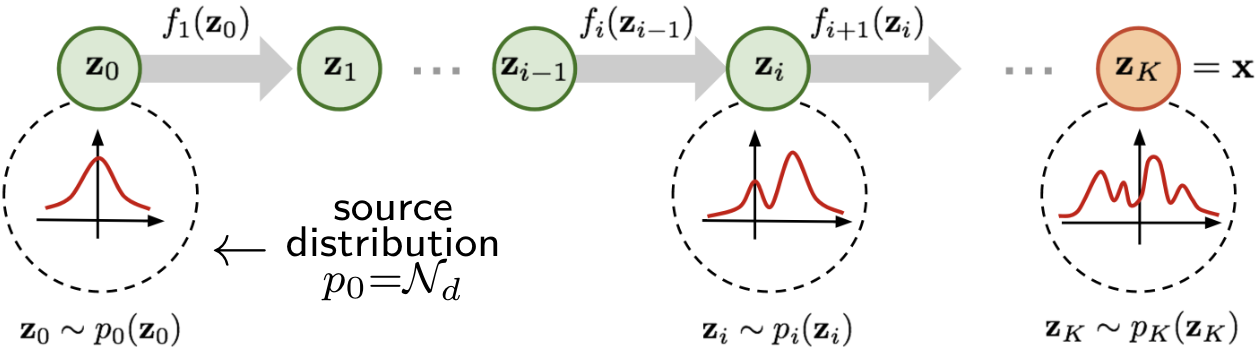
\includegraphics[width=.5\textwidth]{img/nf.png}}

%End of title page configuration block
%------------------------------------------------------------

%The next block of commands puts the table of contents at the 
%beginning of each section and highlights the current section:

\AtBeginSection[]
{
  \begin{frame}
    \frametitle{Outline}
    \tableofcontents[currentsection]
  \end{frame}
}
% ------------------------------------------------------------


\begin{document}

\frame{\titlepage}


%---------------------------------------------------------
% This block of code is for the table of contents after
% the title page
\begin{frame}
\frametitle{Outline}
\tableofcontents
\end{frame}
%---------------------------------------------------------

\section{Dynamic Optimal Transport}

\begin{frame}{Dynamic Optimal Transport ($\nicefrac{1}{2}$)}
	We have explored the following Optimal Transport problem:
	\begin{gather}
		L_{\bm{C}}(a, b) := \min_{\bm{P} \in \mathcal{U}(a, b)} \langle \bm{C}, \bm{P} \rangle_F = \sum_{i, j} \bm{C}_{i,j} \bm{P}_{i, j}
	\end{gather} \pause
	This notion has a couple of properties / constraints:
	\begin{enumerate}[label=\arabic*.]
		\item $\mathcal{U}$ represents the set of valid couplings, which encapsulates criteria:
			\begin{enumerate}[label=\alph*.]
				\item Mass is conserved.
				\item Applying the coupling gets us the target mesures: $\beta = \bm{P}_\sharp \alpha$
			\end{enumerate}
		\item The optimization problem is \textit{convex}.
		\item If $\bm{C}$ is a distance in element space, $L_{\bm{C}}$ is a distance in measure space.
	\end{enumerate} \pause ~\\
	\textbf{Observation:} $\bm{C} = \| \cdot \|_2^2 \implies L_{\bm{C}}$ is \textbf{squared geodesic distance}. \pause \\
	\textbf{Implication:} Solving for Endpoints $\rightarrow$ Interpolatable Transport. \pause \newline \\

	\textbf{How?} Using fluid dynamics!
\end{frame}

\begin{frame}{Dynamic Optimal Transport ($\nicefrac{2}{2}$)}
	The Dynamic\footnote{Adjective AND Noun.} Optimal Transport enables us to borrow fluid dynamics literature, and understand how the measure evolves as \textit{time} progresses:
	\begin{gather}
		\text{Let} \quad \mathcal{X}, \mathcal{Y} \in \mathbb{R}^d, \quad \bm{C}(\bm{x}, \bm{y}) = \| \bm{x} - \bm{y} \|^2 \\
		\text{With measures } \alpha_t \quad \text{s.t.} \quad T_\sharp \alpha_0 = \alpha_1 \quad \forall t \in [0, 1]
	\end{gather} \pause
	We can describe the path in continuous time using by moving $\alpha_t$ along a vector field $v_t$. \pause Infinitesimally, our transport cost can be computed as:
	\begin{gather}
		\| v_t \|_{L^2(\alpha_t)} = \left(\int_{\mathbb{R}^d} \| v_t(\bm{x}) \|^2 d\alpha_t(\bm{x}) \right)^{\nicefrac{1}{2}}
	\end{gather} \pause
	Across time $t$, our net transport cost is:
	\begin{gather}
		W_2^2(\alpha_0, \alpha_1) = \min_{\alpha_t, v_t} \int_0^1 \int_{\mathbb{R}^d} \| v_t(\bm{x}) \|^2~d\alpha_t(\bm{x})~dt
	\end{gather} \pause
	To satisfy mass conservation, we also enforce the following constraint:
	\begin{gather}
		\partial_t \alpha_t + \mathrm{div}(\alpha_t v_t) = 0
	\end{gather}
\end{frame}

\begin{frame}{Mean-Field Games}
	\textbf{Problem:} The mass-conservation constraint, requiring computing $\alpha_t v_t$ makes the problem \underline{non-convex}. \pause \\
	\textbf{Solution:} We can reparameterize the problem using Mean-Field Games:
	\begin{enumerate}[label=\arabic*.]
		\item MFGs are $\infty$-agent games with each agent in spatial domain trying to minimize individual cost. We assume a density function at time $t$. 
			\begin{gather}
				\min_{\alpha_t, v_t} T(\alpha_0, \alpha_1) + \int^1_0 \int_{\mathbb{R}^d} L(\bm{x}, v_t(\bm{x}), \alpha_t(\bm{x}))~dx~dt
			\end{gather} \pause
			\vspace{-.85em}
		\item We define agent trajectories $F: \mathbb{R}^d \times [0, 1] \rightarrow \mathbb{R}^d$ satisfying:
			\begin{gather}
				\begin{cases}
					\partial_t F(\bm{x}, t) = v_t(F(\bm{x}, t)) & \forall \bm{x} \in \mathbb{R}^d,~t \in [0, 1] \\
					F(\bm{x}, 0) = \bm{x}
				\end{cases}
			\end{gather}\pause 
			\vspace{-.85em}
		\item Which under the reparameterization is \textit{convex}:
			\begin{gather}
				\hspace{-2em}
				\min_{\alpha_t, v_t} \int_0^1 \int_{\mathbb{R}^d} \| v_t(x) \|^2~d\alpha_t(x)~dt = \min_{F} \int_0^1 \int_{\mathbb{R}^d} \| \partial_t F(\bm{x}, t) \|^2 \alpha_0(\bm{x}) ~dx~dt
			\end{gather} \pause
	\end{enumerate}
	\vspace{-.85em}
	Next, we need to find a way to learn $F$. Let's talk normalizing flows.
\end{frame}

\section{Normalizing Flows}

\begin{frame}{Generative Modelling Framework}
	\begin{figure}
		\centering
		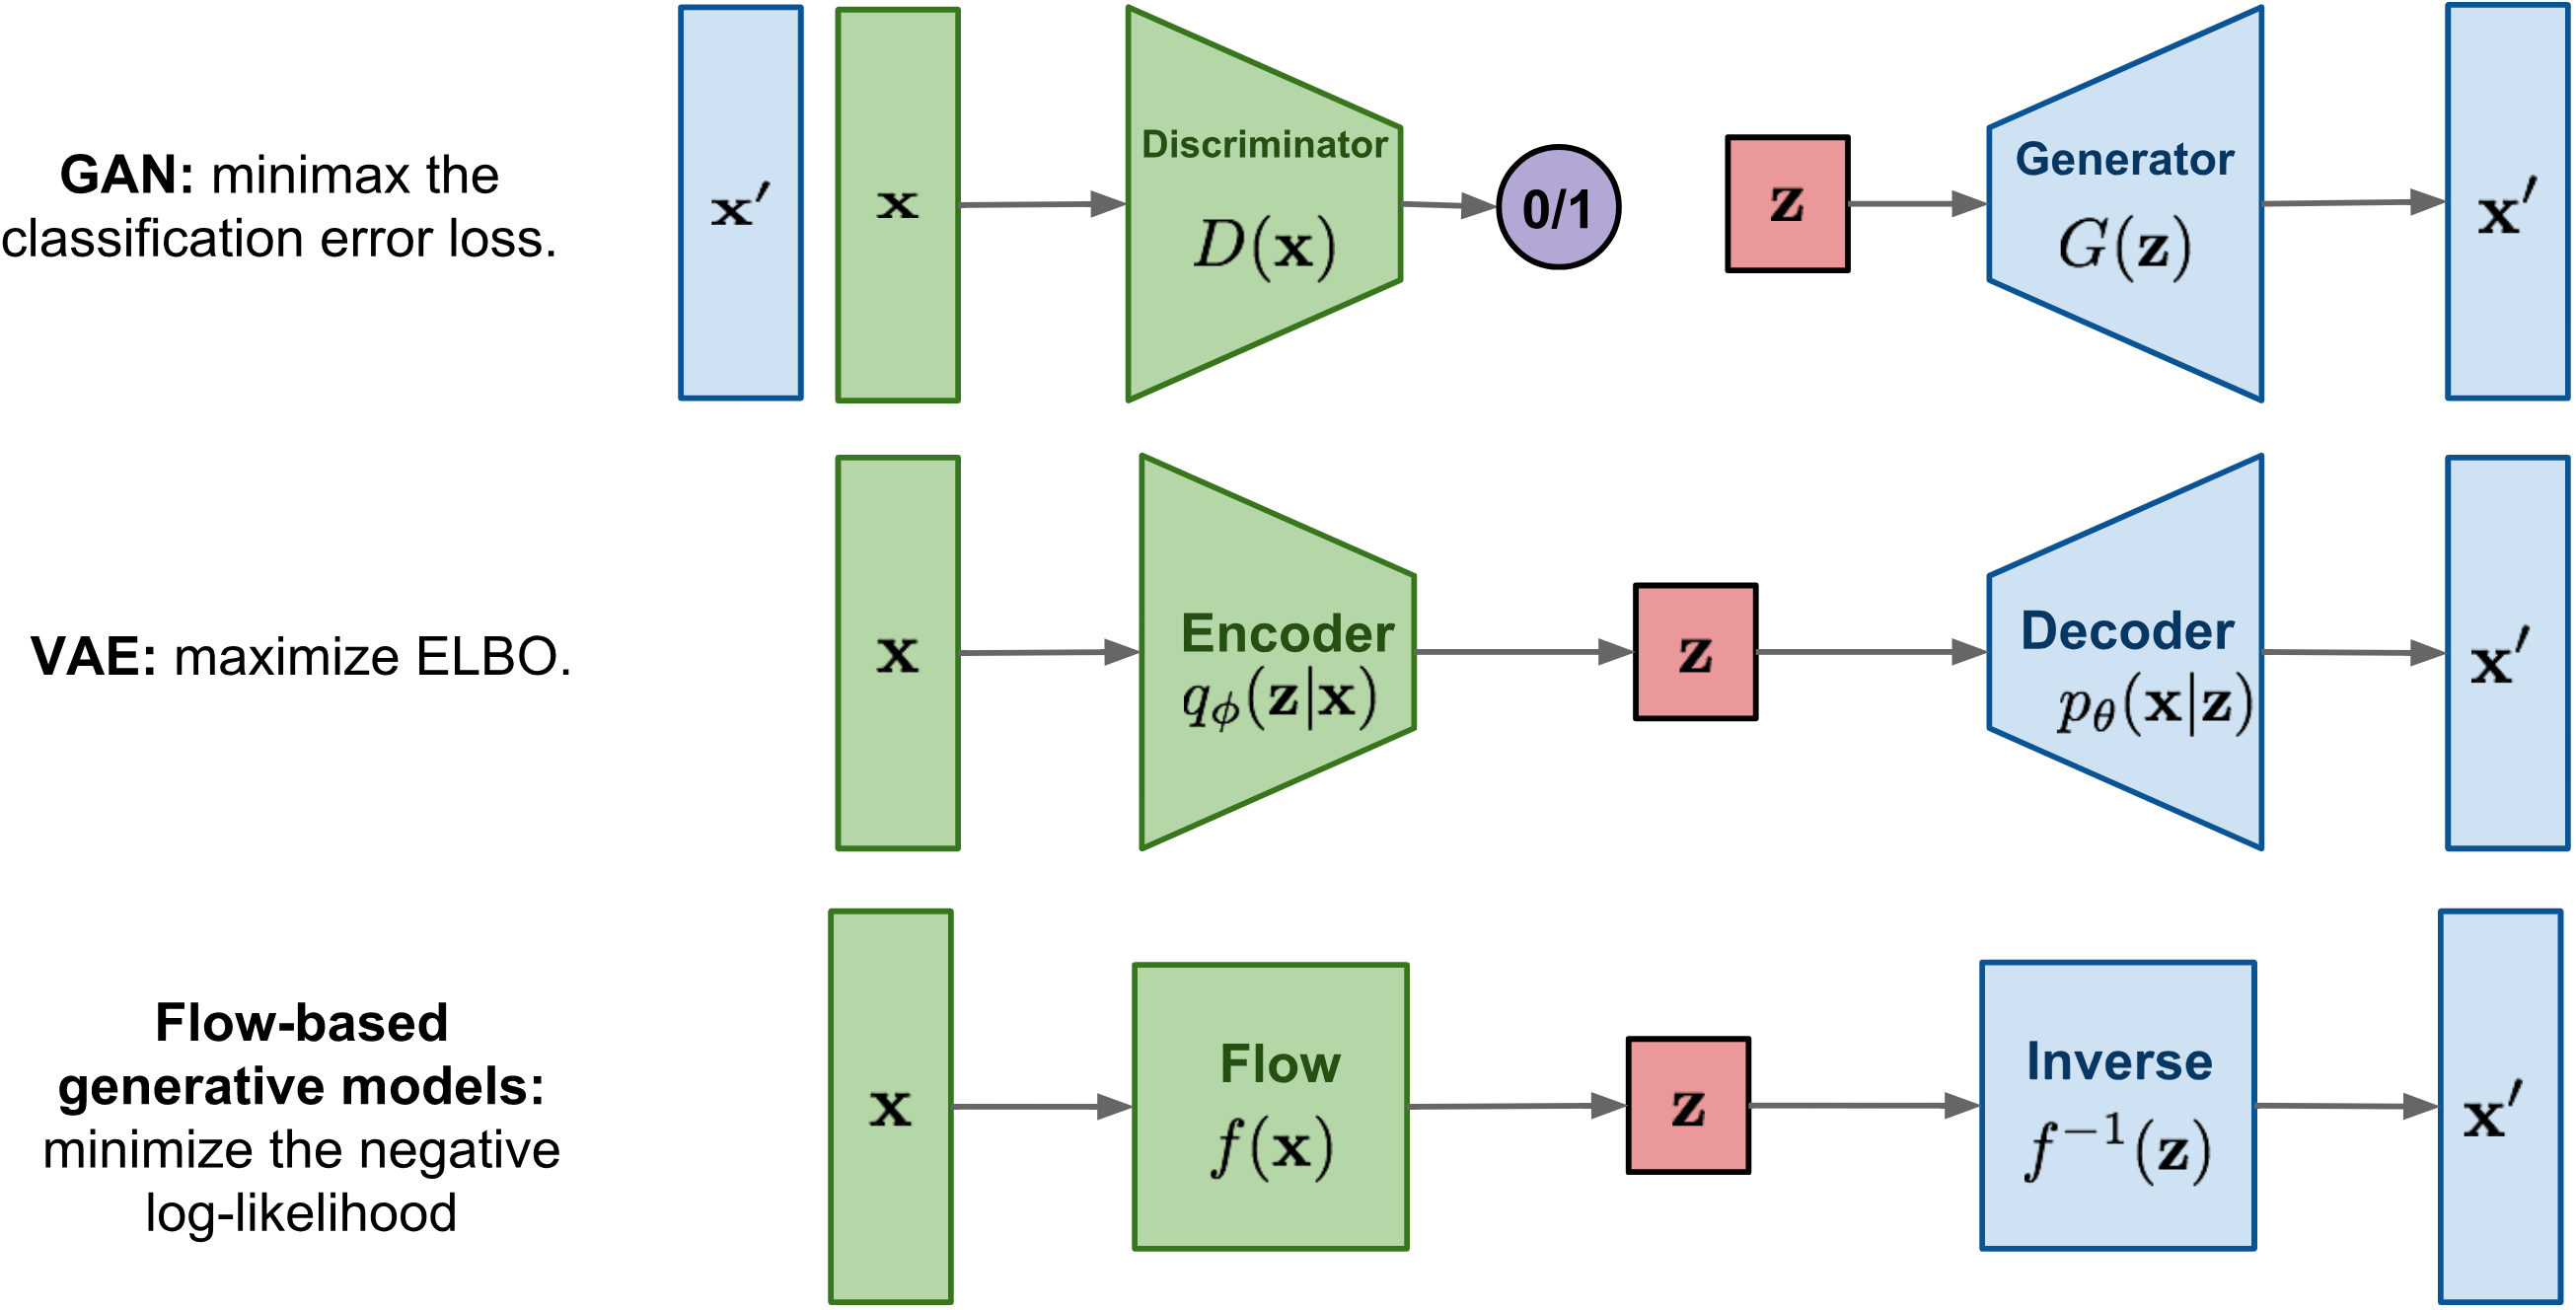
\includegraphics[width=\textwidth]{img/three-generative-models.png}
		\caption{\footnotesize Image Credit: \url{https://lilianweng.github.io/posts/2018-10-13-flow-models/}}
	\end{figure}
\end{frame}

\begin{frame}{Change of Variables}
	Since mass vectors are sampled from $\Sigma$, $\alpha_t$ are \textit{probabibility measures}. \pause \newline \\

	Setting $\bm{y} = T(\bm{x})$, we can apply the change of variables formula:
	\begin{gather}
		\hspace{-.8em}\alpha_1(\bm{y}) = \alpha_0( T^{-1}_\sharp \alpha_1(\bm{y})) | \det \nabla_{\bm{y}} T_\sharp^{-1} \alpha_1(\bm{y}) | = \frac{\alpha_0( T^{-1}_\sharp \alpha_1(\bm{y}))}{|\det \nabla_{\bm{x}} T_\sharp \circ T_\sharp^{-1} \alpha_1(\bm{y})|}
	\end{gather}
	To compute the PDF of $\alpha_1$. \pause \newline \\

	We still need a known $\alpha_0$, so we use the multivariate normal $\mathcal{N}(0, \bm{I})$:
	\begin{gather}
		\alpha_0(x) = \left(\frac{1}{2\pi}\right)^{\nicefrac{d}{2}} \exp\left(-\frac{1}{2} \| \bm{x} \|^2 \right)
	\end{gather} \pause
	Our goal is to learn the \textit{inverse direction} -- a function from target measure $\alpha_1$ to source measure $\alpha_0$. Next, we can discuss approches to model $T$.
\end{frame}

\begin{frame}{Invertible Functions}
	We need three major properties from our choice of model:
	\begin{enumerate}[label=\arabic*.]
		\item Must be invertible, so that we can \underline{learn the normalizing direction}. \pause
		\item Must be expressive enough to model the target distribution. \pause
		\item Must be efficient to compute. \pause
	\end{enumerate}
	The class of functions that satisfies these properties are \textbf{diffeomorphisms}. \pause \newline \\

	Diffeomorphisms are arbitrarily composable. Let $y_{\ell} := f_{\ell}$ be diffemorphisms with inverses $g_{\ell}$ for $\ell \in \{1, \ldots, L\}$:
	\begin{gather}
		F := f_{L} \circ f_{L-1} \circ \cdots \circ f_{2} \circ f_{1} \\
		G := g_{1} \circ g_{2} \circ \cdots \circ g_{L-1} \circ g_{L}
	\end{gather}
	Then we have $F = G^{-1}$. \pause Additionally, we can also compose determinants:
	\begin{gather}
		\det \nabla_{\bm{y}} F = \prod^L_{\ell=1} \det \nabla_{\bm{y}_\ell} f_{\ell}
	\end{gather} \pause
	This is huge for satisfying property 2.
\end{frame}

\begin{frame}{Optimization by Maximum Likelihood}
	Learning Normalizing Flows allows us to directly maximize log-likelihood:
	\begin{gather}
		\min_{\theta} D_{\mathrm{KL}}(\alpha_1 || T_\sharp \alpha_0) = -\mathbb{E}_{\bm{x} \sim \alpha_1}[\log \alpha_0(G(\bm{x})) + \log |\det \nabla_{\bm{y}} G|] + C
	\end{gather}
	With some constant $C$, which for purpose of optimization we can ignore. \pause \newline \\

	\textbf{Caveat:} Models trained using $D_{\mathrm{KL}}$ are volatile to initialization and interpolate poorly:
	\begin{figure}[h]
		\centering

		\begin{minipage}{0.142\linewidth}
			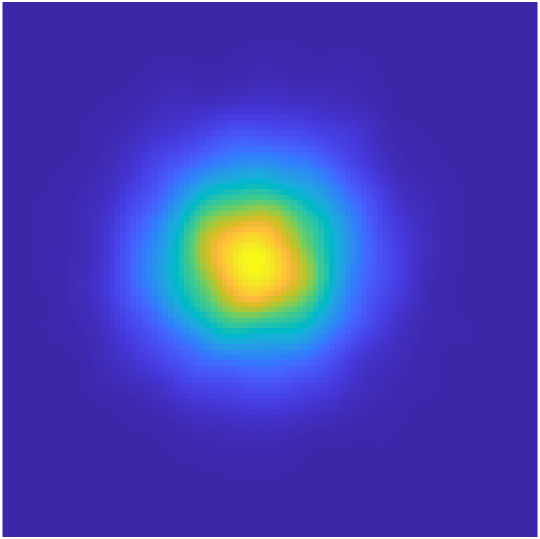
\includegraphics[width=1\linewidth]{img/density_1_RealNVP_S_OT_0.png}\\
		\end{minipage}\hfill
		\begin{minipage}{0.142\linewidth}
			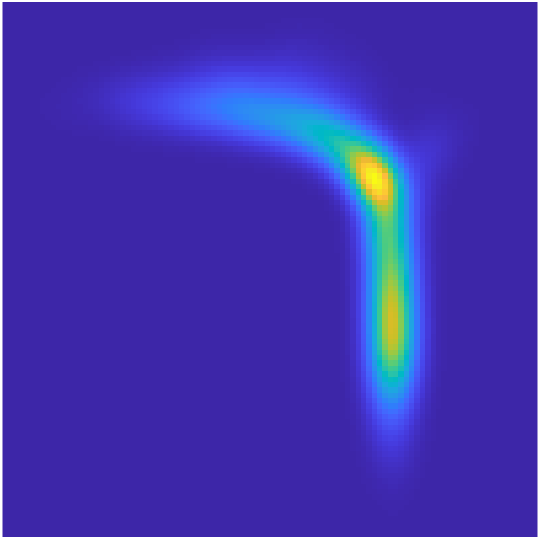
\includegraphics[width=1\linewidth]{img/density_2_RealNVP_S_OT_0.png}\\
		\end{minipage}\hfill
		\begin{minipage}{0.142\linewidth}
			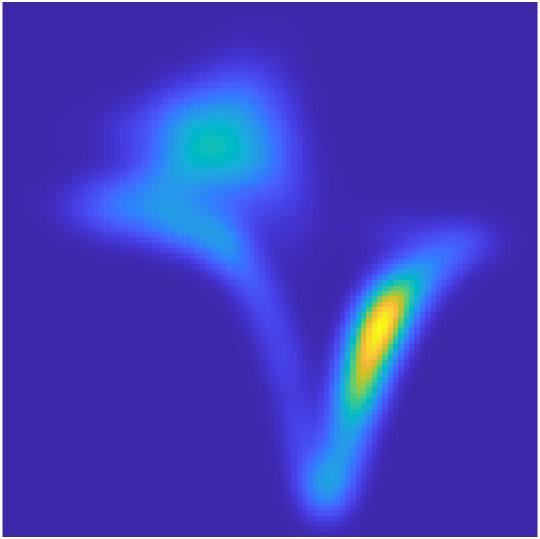
\includegraphics[width=1\linewidth]{img/density_3_RealNVP_S_OT_0.png}\\
		\end{minipage}\hfill
		\begin{minipage}{0.142\linewidth}
			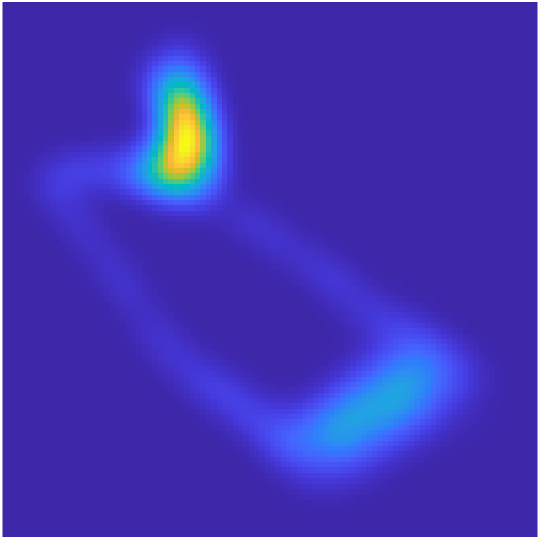
\includegraphics[width=1\linewidth]{img/density_4_RealNVP_S_OT_0.png}\\
		\end{minipage}\hfill
		\begin{minipage}{0.142\linewidth}
			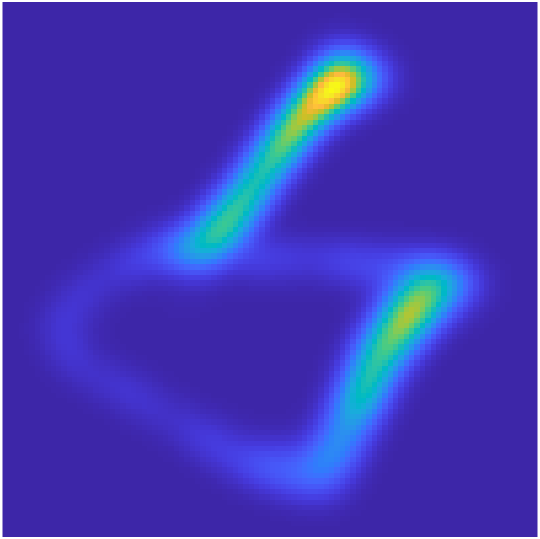
\includegraphics[width=1\linewidth]{img/density_5_RealNVP_S_OT_0.png}\\
		\end{minipage}\hfill
		\begin{minipage}{0.142\linewidth}
			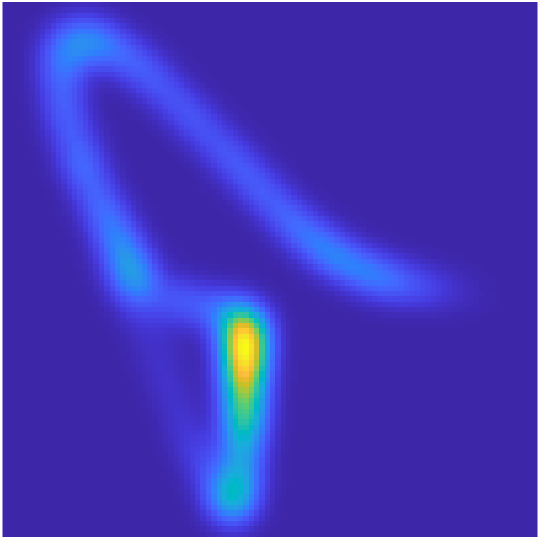
\includegraphics[width=1\linewidth]{img/density_6_RealNVP_S_OT_0.png}\\
		\end{minipage}\hfill
		\begin{minipage}{0.142\linewidth}
			
\includegraphics[width=1\linewidth]{img/density_7_RealNVP_S_OT_0.png}\\
		\end{minipage}\hfill
	\end{figure} \pause
	\vspace{-1em}
	Which we can fix by regularization to transport cost:
	\begin{figure}[h]
		\centering

		\begin{minipage}{0.142\linewidth}
			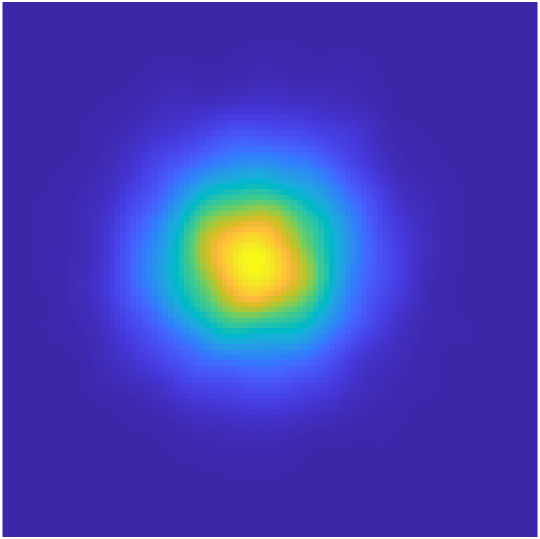
\includegraphics[width=1\linewidth]{img/density_1_RealNVP_S_OT_5e-2.png}\\
		\end{minipage}\hfill
		\begin{minipage}{0.142\linewidth}
			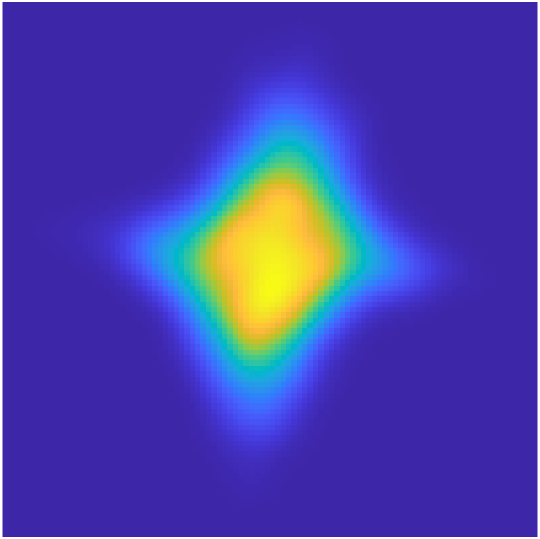
\includegraphics[width=1\linewidth]{img/density_2_RealNVP_S_OT_5e-2.png}\\
		\end{minipage}\hfill
		\begin{minipage}{0.142\linewidth}
			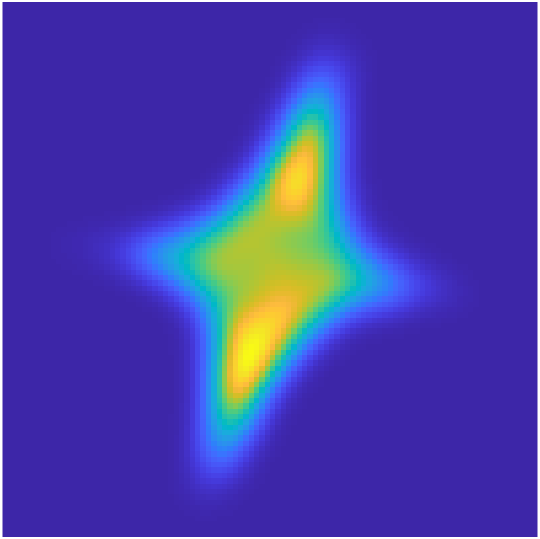
\includegraphics[width=1\linewidth]{img/density_3_RealNVP_S_OT_5e-2.png}\\
		\end{minipage}\hfill
		\begin{minipage}{0.142\linewidth}
			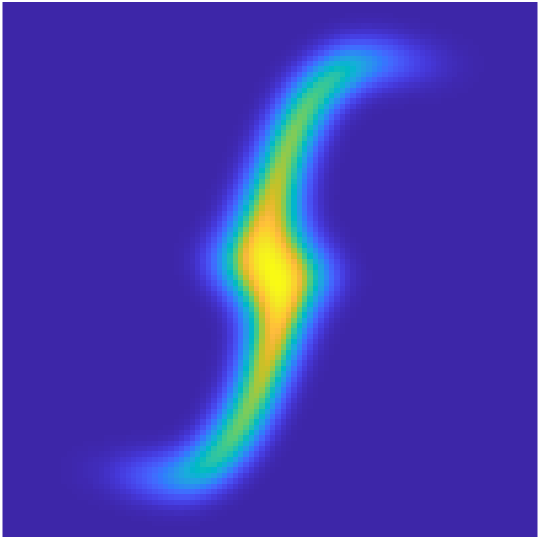
\includegraphics[width=1\linewidth]{img/density_4_RealNVP_S_OT_5e-2.png}\\
		\end{minipage}\hfill
		\begin{minipage}{0.142\linewidth}
			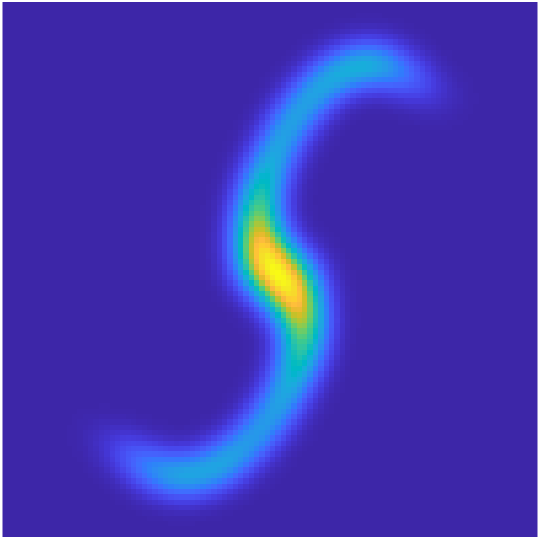
\includegraphics[width=1\linewidth]{img/density_5_RealNVP_S_OT_5e-2.png}\\
		\end{minipage}\hfill
		\begin{minipage}{0.142\linewidth}
			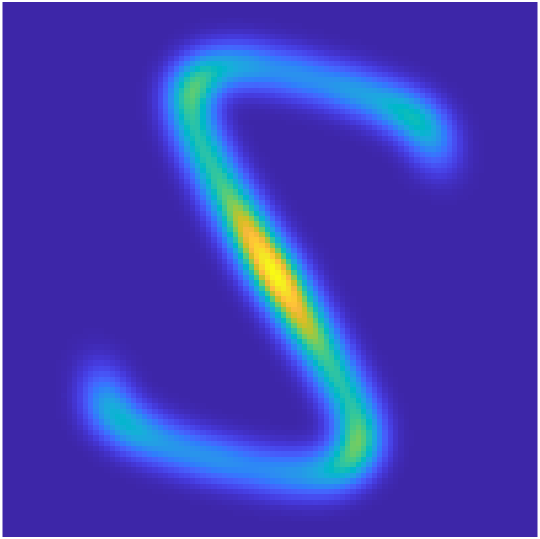
\includegraphics[width=1\linewidth]{img/density_6_RealNVP_S_OT_5e-2.png}\\
		\end{minipage}\hfill
		\begin{minipage}{0.142\linewidth}
			
\includegraphics[width=1\linewidth]{img/density_7_RealNVP_S_OT_5e-2.png}\\
		\end{minipage}\hfill
	\end{figure}

\end{frame}

\begin{frame}{Coupling Flows}
	One clever diffeomorphism is a \textbf{coupling flow}:
	\begin{center}
		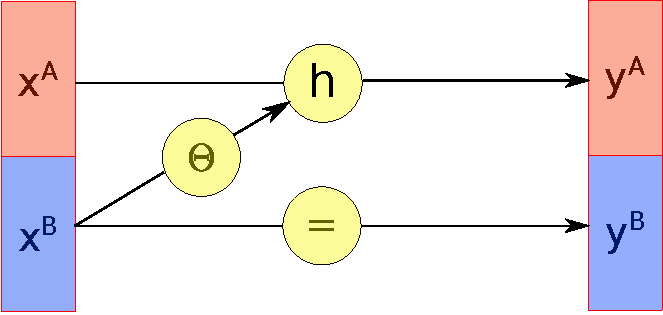
\includegraphics[width=.5\textwidth]{img/coupling_flows}
	\end{center} \pause
	With random permutation $\Pi$, we define forward flow ($\alpha_0 \rightarrow \alpha_1$) as:
	\begin{gather}
		\bm{x}' := \Pi(\bm{x}), \qquad \mathbf{w}, \mathbf{b} := h_\Theta(\bm{x}'_{\nicefrac{D}{2}+1 : D}) \\
		f_k^{(\Theta_k)}(\bm{x}) := \text{Concat}([\bm{x}'_{1:\nicefrac{D}{2}} \odot \exp(\mathbf{w}) + \mathbf{b}, \bm{x}'_{\nicefrac{D}{2}+1:D}])
	\end{gather} \pause
	Subsequently inverse flow ($\alpha_1 \rightarrow \alpha_0$) is defined as follows:
	\begin{gather}
		\mathbf{w}, \mathbf{b} := h_\Theta(\bm{y}_{\nicefrac{D}{2}+1 : D}) \\
		f_k^{(\Theta_k)^{-1}}(\bm{y}) := \Pi^{-1} \left( \text{Concat}([(\bm{y}_{1:\nicefrac{D}{2}} - \mathbf{b}) \oslash \exp(\mathbf{w}) , \bm{y}_{\nicefrac{D}{2}+1:D}]) \right)
	\end{gather}
\end{frame}

\begin{frame}{Computing the $\log | \det (\cdot ) |$}
	Best part, the Jacobian of $f_k^{(\Theta_k)^{-1}}$ has the the following block form:
	\begin{equation}
		\nabla f_k^{(\Theta_k)^{-1}} (\bm{y}) = \begin{bmatrix}
			I_{\nicefrac{D}{2} \times \nicefrac{D}{2}} & \mathbf{0}_{\nicefrac{D}{2} \times \nicefrac{D}{2}} \\
			\frac{\partial f^{(\Theta_k)^{-1}}_{k,\nicefrac{D}{2}+1:D}}{\partial \bm{y}_{1:\nicefrac{D}{2}}} & \text{diag}\left(\exp\left( -\mathbf{w} \right)\right)
		\end{bmatrix} \pause
	\end{equation}
	Which enables us to compute its determinant in linear time:
	\begin{equation}
		\det \nabla f_k^{(\Theta_k)^{-1}}(\bm{y}) = \exp \left( \sum -\mathbf{w}_k \right)
	\end{equation} \pause
	Which we can further use to compute composed $\log \det \nabla F^{-1}$:
	\begin{gather}
		\log \det \nabla F^{-1}(\bm{y}) = \sum^{L-1}_{\ell=0} \sum^{\nicefrac{D}{2}}_{i=1} -\mathbf{w}_i^{(\ell)}
	\end{gather} \pause
	\textbf{Implication:} $h_{\Theta}$ can be arbitrarily complex!
\end{frame}

\section{Transport-Regularized Normalizing Flows}

\begin{frame}{Setting the Terminal Condition}
	The final thing left to discuss is the terminal condition. We need $F$ s.t:
	\vspace{-.5em}
	\begin{gather}
		F(\bm{x}, 1) = \bm{y} \sim \alpha_1 \quad \forall x \in \mathbb{R}^d
	\end{gather} \pause
	Instead of solving a constrained problem, we soft-constraint using $D_{\mathrm{KL}}$:
	\vspace{-.5em}
	\begin{gather}
		\min_{F} \int_0^1 \int_{\mathbb{R}^d} \| \partial_t F(\bm{x}, t) \|^2 \alpha_0(\bm{x}) ~dx~dt + \lambda D_{\mathrm{KL}}(\alpha_1 || F_\sharp \alpha_0)
	\end{gather}
	$D_{\mathrm{KL}}$ is conventional cost; we just add transport cost, hence new formulation is called \textbf{transport-regularized normalizing flows}. \pause \newline \\

	Discretizing across a composition of $L$ flows, we have:
	\vspace{-.5em}
	\begin{gather}
		\min_{F} L \cdot \mathbb{E}_{\bm{x} \sim \alpha_0} \left[ \sum^{L - 1}_{\ell = 0} \| F_{\ell + 1}(\bm{x}) - F_{\ell}(\bm{x}) \|_2^2 \right] + \lambda D_{\mathrm{KL}}(\alpha_1 || F_\sharp \alpha_0)
	\end{gather}
	Using this, we can train transport-regularized normalizing flows.
\end{frame}

\begin{frame}{Implementation Details}
	\begin{center}
		If you can view this screen, I am making a mistake.
	\end{center}
\end{frame}

\begin{frame}{Thank you!}
	\begin{center}
		Have an awesome rest of your day!
	\end{center}
	\begin{center}
		\textbf{Slides:} \url{https://jinen.setpal.net/slides/nf.pdf}
	\end{center}
\end{frame}

\end{document}
